\begin{pastexam}[label={px:ntut-114-ee-ds-06}]{北科大電機所（戊組） 114 學年度 第 II-2 題}
（簡答；4 分）

Given a binary search tree in \textbf{Fig. 1}, insert 30, 45, 75, 85, 95, and 65 (in this order) into the
binary search tree. What is the pre-order traversal? \textbf{(4\%)}

\begin{center}
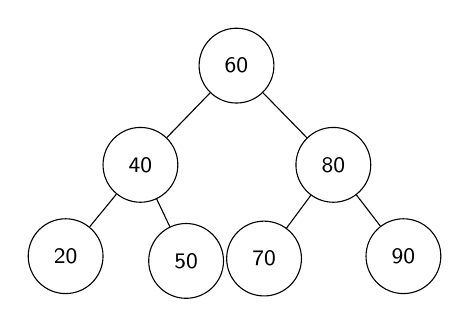
\begin{tikzpicture}[n/.style={circle,draw,fill=white,inner sep=0pt,minimum size=9.5mm,font=\footnotesize\sffamily}]
\node[n] (n60) at (2.17,0.00) {60};
\node[n] (n40) at (0.95,-1.26) {40};
\node[n] (n80) at (3.40,-1.26) {80};
\node[n] (n20) at (0.00,-2.42) {20};
\node[n] (n50) at (1.53,-2.48) {50};
\node[n] (n70) at (2.52,-2.45) {70};
\node[n] (n90) at (4.29,-2.42) {90};
\draw (n60)--(n40);
\draw (n60)--(n80);
\draw (n40)--(n20);
\draw (n40)--(n50);
\draw (n80)--(n70);
\draw (n80)--(n90);
\end{tikzpicture}\\[2pt] \textbf{Fig. 1}
\end{center}
\end{pastexam}

\begin{pastsoln}
答：60, 40, 20, 30, 50, 45, 80, 70, 65, 75, 90, 85, 95。

每個鍵從根往下比，小的往左、大的往右，走到空位就放下（資結書第~9.2~節）：
\begin{itemize}
\item 30：$< 60$ 往左，$< 40$ 往左，$> 20$，放在 20 的右邊。
\item 45：$< 60$，$> 40$，$< 50$，放在 50 的左邊。
\item 75：$> 60$，$< 80$，$> 70$，放在 70 的右邊。
\item 85：$> 60$，$> 80$，$< 90$，放在 90 的左邊。
\item 95：$> 60$，$> 80$，$> 90$，放在 90 的右邊。
\item 65：$> 60$，$< 80$，$< 70$，放在 70 的左邊。
\end{itemize}
\begin{center}
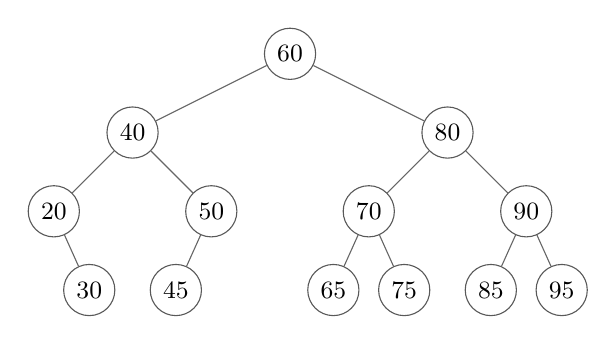
\begin{tikzpicture}[
    btn/.style={circle, draw=black!65, line width=0.4pt, minimum size=6.5mm, inner sep=0pt, font=\small},
    level distance=10mm, edge from parent/.style={draw=black!60},
    level 1/.style={sibling distance=40mm}, level 2/.style={sibling distance=20mm},
    level 3/.style={sibling distance=9mm}]
\node[btn] {60}
    child {node[btn] {40}
        child {node[btn] {20} child[missing] child {node[btn] {30}}}
        child {node[btn] {50} child {node[btn] {45}} child[missing]}}
    child {node[btn] {80}
        child {node[btn] {70} child {node[btn] {65}} child {node[btn] {75}}}
        child {node[btn] {90} child {node[btn] {85}} child {node[btn] {95}}}};
\end{tikzpicture}
\end{center}
前序（根、左、右）：先根 60；左子樹 40、20、30、50、45；右子樹 80、70、65、75、90、85、95。 合起來是
60, 40, 20, 30, 50, 45, 80, 70, 65, 75, 90, 85, 95。
\end{pastsoln}
